%COMPILATION: 
%clear; bibtex main.aux;pdflatex main.tex ;evince main.pdf &

\chapter{Introduction}                   		% chapter 1 
	\section{Contexte et objectif}

	Les travaux présentés dans ce document ont été réalisés au cours d'un stage de master recherche de cinq mois qui s'est déroulé au sein du laboratoire LISA de l'école d'ingénieur ISTIA à Angers. Plus particulièrement dans le contexte de l'activité de recherche de l'analyse d'images pour l'aide au diagnostic. Il fait suite à une recherche bibliographique sur ``l'interprétation d'images et graphe conceptuel intégrant des connaissances topologiques et photométriques''. 
	
	L'objectif de ce stage est d'utiliser des notions conceptuelles non quantitatives, topologiques et photométriques, pour l'interprétation d'images synthétiques puis médicales.
	Le bénéfice attendu est d'optimiser la segmentation et le fenêtrage\footnote{Le fenêtrage est le fait de considérer qu'une fraction de la dynamique d'une image (e.g. une section d'un histogramme d'image), on l'utilise souvent pour faciliter la visualisation ou les traitements d'une image.} (rendu visuel) d'une région d'intérêt (e.g. tumeur).
	
	%Il est le fruit d'une centaine d'heures de documentation et de réflexion sur l'intégration de connaissances spatiales (e.g. distance, topologie \footnote{La topologie est une branche des mathématiques concernant l'étude des déformations spatiales par des transformations continues (sans arrachages ni recollement des structures)\url{http://fr.wikipedia.org/wiki/Topologie}.}) et photométriques pour l'interprétation des images (i.e. segmentation et identification de régions). L'objectif est d'intégrer ce type de notion conceptuelle ou abstraite en privilégiant celles qui ne sont pas quantitatives (topologie, relation d'intensité non quantitative). Le bénéfice attendu est de faciliter le paramétrage d'algorithmes utilisés pour l'interprétation d'images et la réduction de l'espace de recherche (ex. région d'intérêt). Ce travail fait suite aux travaux de M.Fasquel \cite{Fasquel2006} qui se limitait aux informations topologiques, avec pour application l'analyse d'images médicales pour l'aide au diagnostic.

%{\bf Trop particulier: pour des actes diagnostic spécifique (recherche de tumeur...)}

%{\bf La phrase "Ces connaissances sont souvent représentées sous forme de graphe conceptuel." a été retirée car trop spécifique (éventuellement à placer ailleurs).}

% , sur l'interprétation séquentielle d'images et de graphes conceptuels pour l'optimisation du fenêtrage \footnote{Le fenêtrage est le fait de considérer qu'une fraction de la dynamique d'une image (exemple : un intervalle dans un histogramme d'image), on l'utilise souvent pour faciliter la visualisation ou les traitements d'une image.} d'images médicales. Ce fenêtrage pourra être effectué au moyen d'un logiciel permettant à l'utilisateur d'interagir avec des images numériques.
%Le thème est original par la combinaison de deux bases de connaissances à priori indépendantes, à caractère topologique et photométrique. Il fait suite aux travaux de M.Fasquel \cite{Fasquel2006}. Le cadre général est le développement de méthodes et d'outils d'assistance au diagnostic.

	\section{Problématique}
	
	Nous proposons d'interpréter des images en combinant des informations topologiques \cite[Fasquel]{Fasquel2006} et photométriques non quantitatives. Un exemple de situation où ce type d'information pourrait être avantageusement exploité serait celui illustré par la figure~\ref{fig:sl_0_1}. Cet exemple concerne le rendu volumique d'une image médicale. Le choix de la fenêtre de rendu (une plage d'intensités à afficher) est crucial pour améliorer la perception d'une structure donnée. Dans ce cas, on cherche à rendre le réseau vasculaire, supposant que l'on dispose du masque des os. Sachant que le réseau vasculaire n'est pas inclus dans les os (information topologique à priori), on peut tout simplement retirer de l'image le volume relatif au os afin de faciliter la visualisation du réseau vasculaire (figure~\ref{fig:sl_0_2}). Par ailleurs, dans l'hypothèse où le réseau vasculaire est plus clair que le tissu du foie (information photométrique que l'on retrouve visuellement sur la figure~\ref{fig:sl_0_2}), on peut modifier le fenêtrage de manière à afficher que les tissus qui ont une intensité supérieure à ceux du foie (voir figure~\ref{fig:sl_0_3}).

	%%%%%%%%%%%%%%%%%%%%%%%%%%%%%%%%%%%%%%%%%%%%%%%%
	\begin{figure}[!ht]	%trim=l b r t  width=0.5\textwidth, 
	  \centering
		\subfloat[Rendu initial]{\label{fig:sl_0_1}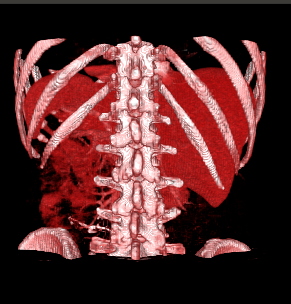
\includegraphics[trim= 0mm 15mm 0mm 10mm, clip, height=0.24\textwidth]{Introduction/figure/sl_0_1.png}}					\hspace{0.4em}
		\subfloat[Rendu intermédiaire (masquage)]{\label{fig:sl_0_2}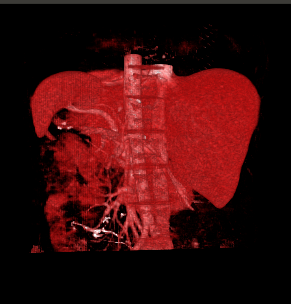
\includegraphics[trim= 0mm 15mm 0mm 15mm, clip, height=0.24\textwidth]{Introduction/figure/sl_0_2.png}}	\hspace{0.4em}
		\subfloat[Rendu optimal (fenêtrage)]{\label{fig:sl_0_3}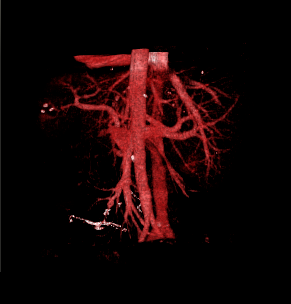
\includegraphics[trim= 5mm 20mm 5mm 15mm, clip, height=0.24\textwidth]{Introduction/figure/sl_0_3.png}}
		\caption{Rendu manuel du réseau vasculaire}
	\end{figure}
	%%%%%%%%%%%%%%%%%%%%%%%%%%%%%%%%%%%%%%%%%%%%%%%%
	
%\newpage
	Cet exemple peut nous amener à nous poser les questions suivantes :\vspace{1 em}

	Si l'on considère une image en niveaux de gris, contenant une région $A$ et une région $B$ comme sur la figure~\ref{fig:structure_a_b}, comment représenter et utiliser, pour l'interprétation automatique d'images, des concepts non quantitatifs tels que :


	\begin{itemize}
		\item La région $A$ recouvre-t-elle la région $B$ (topologie)?
		\item La région $A$ est-elle plus claire que la région $B$ (photométrie)?
	\end{itemize}
\vspace{1em}

Quels en sont les bénéfices?


	\begin{figure}[!ht]
	  \centering
	      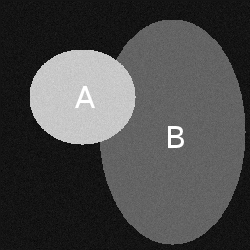
\includegraphics[width=0.2\textwidth]{Introduction/figure/structures_a_b.png}
	  \caption{Représentation synthétique des régions.}
	  \label{fig:structure_a_b}
	\end{figure}


	On s'intéressera à ces questions dans le cas d'un processus d'interprétation séquentiel de l'image où chaque étape conduira à la compréhension d'une région de l'image (i.e. segmentation et identification). Compte tenu de ces questions, la problématique de notre travail peut être modélisée par la figure suivante : 
	%\les aspects sous-jacents à traiter concernent:\\
	
	\begin{figure}[!h]
	\setlength{\unitlength}{1mm}
	\begin{center}
	\begin{picture}(60,40)
		\put(-10,0){\framebox(80,10){Guidage du traitement de l'image}}
		\put(30,15){\vector(0,-2){5}} 
% 		\put(30,10){\vector(0,0){5}} 
		\put(-10,15){\framebox(80,10){Moteur d'inférence (déduction)}}
		\put(40,30){\vector(0,-2){5}}
		\put(20,30){\vector(0,-2){5}}
% 		\put(30,25){\vector(0,0){5}}  
		\put(32,30){\framebox(90,10){Modélisation du processus de segmentation}}
		\put(-62,30){\framebox(90,10){Représentation des informations conceptuelles}}
	\end{picture}
	\end{center}
	\caption{Problématique et entités associées.}
	\label{pic:process1}
	\end{figure} 


%	\begin{itemize}
%	\item La représentation de ces informations
%	\item La modélisation du processus de segmentation
%	\item Les inférences (déductions à partir du graphe portant sur la région d'intérêt et les classes)
%	\item L'utilisation pour guider le traitement de l'image \\
%	\end{itemize}

%	La problématique de notre travail est modélisée par la figure suivante : \\

	  \section{État de l'art}
	  \label{sec:state_of_the_art}

	%%%%%%%%%%%%%%%%%%%%%%%%%%%%%%%%%%%%%%%%%%%%%%%%%%%%%%%%%%%%%%%%%%%%%%%%%%%%%%%%%%%%%%%%%%%%%%%%%%%%%%%%%%%%%%%%%%%%%
	%													État  de l'art													%
	%%%%%%%%%%%%%%%%%%%%%%%%%%%%%%%%%%%%%%%%%%%%%%%%%%%%%%%%%%%%%%%%%%%%%%%%%%%%%%%%%%%%%%%%%%%%%%%%%%%%%%%%%%%%%%%%%%%%%
		\subsubsection*{Stratégie d'analyse d'image}
	Plusieurs approches de segmentations automatiques d'images ont déjà ét{\bf é} mises à l'épreuve. La première consiste à considérer l'image dans son ensemble. L'idée est de concevoir un seul algorithme permettant de segmenter toutes les structures d'une image \citep[Moreno]{Moreno2008}\citep[Kobashi]{Kobashi1995}. Il est néanmoins courant que toutes les régions d'une images ne puissent pas être segmentées avec un seul algorithme. Il est donc souvent plus réaliste de concevoir un algorithme spécifique à chacune des structures : c'est l'approche séquentielle ou itérative. Elle consiste à segmenter les structures les une après les autres avec un algorithme spécifique à chacune d'elles. Pour segmenter une structure donnée, il est pertinent de s'appuyer sur les informations relatives aux structures préalablement segmentées. Typiquement, il peut s'agir de l'intégration d'une région d'intérêt permettant de délimiter une zone de recherche pour la structure à segmenter \citep[Hudelot]{Hudelot2008}\citep[Fasquel]{Fasquel2006}.


		\subsubsection*{Informations conceptuelles}
	L'utilisation d'informations à priori est un moyen d'anticiper le contenu d'une image et donc d'en optimiser son traitement. En analyse d'image guidée par des informations à priori abstraites, les travaux récemment réalisés se focalisent sur des informations spatiales. Il peut s'agir de relations entre les structures de type topologiques (e.g. inclusion, recouvrement, adjacence) \citep[Fasquel]{Fasquel2006}\citep[Egenhofer]{Egenhofer2009}\citep[Hudelot]{Hudelot2008} ou bien relatives à des notions de direction et de distance \citep[Hudelot]{Hudelot2008}. Un inconvénient des informations de distance et de direction est leurs aspects quantitatifs. Ceci implique la détermination de paramètres qui doivent être adaptés à l'application considérée. Ceci est notamment le cas des récents travaux de \citep[Hudelot]{Hudelot2008}, ou les informations de distance et de direction sont manipulées en utilisant la logique floue, ceci induisant une phase d'apprentissage \textit{``fuzzy model learning''}.


	Ces représentations conceptuelles (ontologiques\footnote{L'ontologie constitue en soi un modèle de données représentatif d'un ensemble de concepts dans un domaine, ainsi que des relations entre ces concepts. ``L'ontologie est aux données ce que la grammaire est au langage'' \url{http://fr.wikipedia.org/wiki/Ontologie_(informatique)}} \citep[Atif]{Atif2007}) sont encore peu étudiées en interprétation d'image \textit{``the development of ontology-based methods for image interpretation is still in its infancy''} \citep[Hudelot, p.1929]{Hudelot2008}. Il demeure une difficulté majeure lors de leurs applications au niveau des algorithmes d'analyses d'images : \textit{``there still exists a large gap between the semantic interpretation of a medical image and its low-level features'' } \citep[Deruyver, p.1245]{deruyver2009}. Comme récemment souligné dans \citep[Hudelot]{Hudelot2008}, ce type de connaissance est généralement utilisé dans des contextes différents de l'interprétation d'images, tel que l'annotation d'images. 

	A notre connaissance, il n'y a pas eu de travaux relatifs à l'analyse d'images guidée par le couplage d'informations conceptuelles topologiques et photométriques non quantitatives, ceci constituant une première originalité de l'orientation de nos travaux.


	\section{Organisation de l'étude}

	L'étude est organisée selon trois aspects correspondant aux volets : formalisation, évaluation et application. 
Le premier aspect (chapitre 2) est dédié à la formalisation en matière de représentation des connaissances et du moteur d'inférence. En ce qui concerne le moteur d'inférence, il s'agit d'établir les relations permettant de déduire, à partir de connaissances à priori sur l'image, des informations bénéfiques au traitement de l'image. 

Le second aspect (chapitre 3) se focalise sur l'évaluation des bénéfices des informations déduites, dans le cas d'un algorithme particulier, le {\it K-Means clustering}, couramment utilisé en traitement d'images.
Le dernier aspect (chapitre 4) est dédié à l'illustration du bénéfice de ce travail dans un cadre applicatif bien particulier relatif à la visualisation d'images médicales.


%	Nous nous limiterons à deux cas d'utilisations pour appuyer cette étude:
%	\begin{itemize}
%		\item l'interprétation d'images synthétiques ;
%		\item la visualisation optimale d'images médicales par un processus de segmentation interactif. \\
%	\end{itemize}

	%Dans ces deux cas d'utilisations, l'algorithme d'analyse d'images sera basé sur une méthode d'analyse d'histogramme classique à partir duquel on identifiera les différentes régions de l'image (voir figure~\ref{fig:melange}). Le cas de l'interprétation d'images synthétiques a principalement pour objectif d'illustrer la problématique, les différents concepts impliqués, la solution proposée {\bf et d'en évaluer quantitativement les bénéfices}.
%	Dans ces deux cas d'utilisations, l'algorithme d'analyse d'images sera basé sur une méthode classique de partitionnement de points selon leurs intensités et correspondants à différentes structures anatomiques et pathologiques\footnote{La pathologie est l'étude des maladies et de leurs causes. Le terme peut être employé comme un nom pour désigner une anomalie dans un corps.} (voir le schéma figure~\ref{fig:melange}). 
	
%	Le premier cas a principalement pour objectif d'illustrer la problématique, les différents concepts impliqués, la solution proposée et d'en évaluer quantitativement les bénéfices.

%Pour cela, il est nécessaire de reconnaître automatiquement la structure d'intérêt au sein de l'image. Nous présenterons les méthodes de traitement d'image existantes, dans le chapitre suivant.


%	\begin{figure}[!ht]
%	  \centering
%	      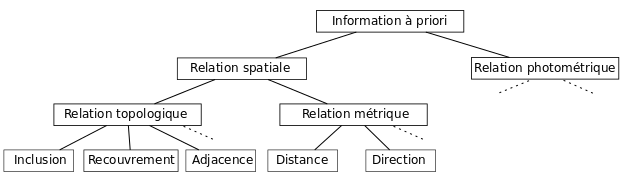
\includegraphics[width=0.9\textwidth]{Introduction/figure/information_a_priori.png}
%	  \caption{Classification des informations conceptuelles.}
%         \label{fig:information_a_priori}
%	\end{figure}

%		\subsubsection*{Informations conceptuelles: représentation}
%		\label{sec:info_concept_reps}
%	La représentation des connaissances, en particulier spatiales, peut se baser sur un graphe (conceptuel lorsque l'on parle de connaissances conceptuelles) où les noeuds sont associés aux différentes entités supposées présentes dans l'image. Les arcs reliant les noeuds représentent les relations (e.g. à gauche, à droite, inclus). Ce type de représentation a notamment été récemment considéré par \citep[Deruyver, p.1246]{deruyver2009} et \citep[Fasquel]{Fasquel2006} et facilite la compréhension : ``\textit{Graph techniques permit to represent image objects and scenes in very natural way}'' \citep[Sanfeliu]{Sanfeliu2002}.


%		\subsubsection*{Informations conceptuelles, contextuelles et interprétation séquentielle}
%	Ces informations conceptuelles à priori peuvent être enrichies tout au long du traitement de l'image. Dans \citep[Fasquel]{Fasquel2006}, ces informations deviennent alors contextuelles : les informations à priori, très générales, deviennent davantage spécifique à l'image en cours d'analyse. Les informations contextuelles évoluent en fonction du contexte dans lequel se trouve une image à un moment donné. Par exemple, lors de la segmentation d'une image, les structures déjà segmentées ou encore le nombres de classes (non pas en général, mais compte tenu des structures déjà identifiées), sont des informations contextuelles. Pour représenter cette évolution des connaissances (i.e. connaissances à priori enrichies par les connaissances contextuelles), on peut intégrer la notion d'activation de noeud du graphe conceptuel initial, comme considéré récemment par \citep[Fasquel]{Fasquel2006}.


%	\section{Analyse d'images par seuillage d'histogramme}		%Information photométrique
%	\label{sec:ana_img_by_threshold}
%	Comme ceci a été précisé lors de la présentation de la problématique générale, nous nous limiterons essentiellement à une analyse d'images basée sur le seuillage d'histogramme\footnote{L'histogramme d'une image est un graphique qui associe les niveaux de gris au nombre de pixel dans l'image qui contient ces niveaux de gris.}. Ce choix est notamment justifié par la nature des informations conceptuelles que nous proposons d'étudier, en particulier l'information photométrique. L'information topologique, quand à elle, interviendra pour réduire le calcul de l'histogramme au sein d'une région d'intérêt, afin d'éliminer les données qui pourraient altérer son analyse (e.g. les données correspondant aux régions déjà segmentées).

%	Nous ne prétendons pas, et ce n'est pas l'objectif de cette étude, proposer une méthode de seuillage d'histogramme nouvelle. Il est néanmoins intéressant de souligner qu'il s'agit d'une catégorie d'algorithme couramment utilisés en traitement d'images, et qui font encore  aujourd'hui l'objet d'études afin d'améliorer leur robustesse. Nous en rappelons ci-dessous succinctement le principe et les limitations couramment rencontrées.

%	Le principe du seuillage\footnote{Le seuillage d'image est la méthode la plus simple de segmentation d'image. À partir d'une image en niveau de gris, le seuillage d'image peut être utilisé pour créer une image comportant uniquement deux valeurs, noir ou blanc (monochrome). \url{http://fr.wikipedia.org/wiki/Seuillage_d'image}} d'histogramme consiste à dire qu'un ensemble de pixels, d'une même image, dont l'intensité est comprise dans un certain intervalle, appartiennent à une structure donnée. Il apparaît donc les notions de seuil minimum et maximum de l'intervalle. Plusieurs études sur les méthodes de seuillage d'histogramme d'image ont été réalisées mais il demeure un problème de robustesse lors de la détermination des seuils (\citep[Coudray]{Coudray2010}, \citep[Bhattacharyya]{Bhattacharyya2011}, \citep[Cheng]{Cheng1998}, \citep[Cuevas]{Cuevas2010}). Le lecteur pourra également se référer à l'état de l'art de \citep[Zhang]{Zhang2008} sur ces méthodes.\vspace{1 em}

%	Une des méthodes célèbres à deux niveaux et celle de \citep[Otsu]{Otsu1979} qui déterminent un seuil entre deux classes considérées donc comme l'objet et le fond de l'image.  Il en résulte une image avec deux classes (souvent noir et blanc) dite \textit{``binaire''}. Travailler avec des images binaires est plus simple et donc plus rapide qu'avec des images en niveau de gris car il n'y a que deux couleurs à considérer. Notons tout de même qu'il y a une importante perte d'information par ce fait mais qu'elle peut être négligée si les seuils sont bien choisis. Des extensions récentes, multi-niveaux, existent \citep[Huang 2009]{Huang2009}. Cette même catégorie a été récemment illustré par  \citep[Cuevas]{Cuevas2010} qui considère plusieurs classes inconnues dans l'image et trouve les seuils qui les bornes. D'autre part, il existe des algorithmes de mélange gaussien \textit{``gaussian mixture''} \citep[Gupta]{Gupta1998} (qui ont par ailleurs fait l'objet d'une récente extension \citep[Huang]{Huang2008}), qui permettent d'estimer les paramètres des courbes de Gauss figure~\ref{fig:gauss_mix} (souvent caractéristique de la répartition des intensités d'une structure quelconque).  Nous l'utiliserons dans ce travail.

%	Dans le cas de cet algorithme couramment utilisé, un élément important concerne la connaissance à priori du nombre de classes (ou régions photométriquement distinctes) présentes dans l'image. Ceci détermine le nombre de lobes présentes dans l'histogramme. Un second élément concerne \textit{``l'identité''} ou \textit{``l'étiquette''} de la région associée à chacun de ces lobes. Par exemple, dans le cas d'images médicales anatomiques, il peut s'agir d'associer correctement un lobe donné de l'histogramme à une structure anatomique particulière. L'objectif du travail effectué sera de déterminer automatiquement le nombre de lobes et leurs identités. Ceci se fera par inférence sur la représentation conceptuelle des connaissances à priori et contextuelles. Par rapport à l'application médicale visée, ces informations pourront être utilisées pour déterminer automatiquement le fenêtrage à considérer.


%	\begin{figure}[!ht]
%	  \centering
%	      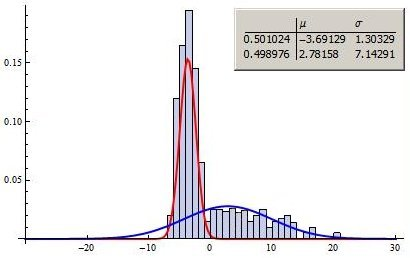
\includegraphics[width=0.5\textwidth]{Introduction/figure/gauss_param.jpg}
%	  \caption{Estimation de gaussiennes.}
%         \label{fig:gauss_mix}
%	\end{figure}

%\newpage

%	\section{Synthèse}
%	Compte tenu de notre connaissance des travaux existants présentés précédemment, l'originalité de nos travaux concernent principalement les trois points suivants :
%	\begin{itemize}
%		\item
%		l'intégration des connaissances photométriques au modèle existant proposé par \citep[Fasquel]{Fasquel2006};
%		\item
%		l'établissement des relations (inférence) entre cette représentation conceptuelle des connaissances et les paramètres quantitatifs d'un seuillage d'histogramme fondé sur le modèle de mélange de gaussiennes. Ces relations concerneront le nombre de classes attendues dans l'image à un instant \textit{t}, puis la détermination de leurs \textit{``étiquettes''};
%		\item
%		l'illustration de l'intérêt de cette approche pour une application particulière : le fenêtrage d'images médicales.
%	\end{itemize}

